\chapter{Surface water map for Murray-Darling River Basin, Australia}
\label{ch7}

\begin{abstract}
This chapter studies derivation of a surface water map of the Murry-Darling River Basin, Australia. Three surface maps are derived from three datasets: Landsat 8, 30m DEM (\gls{SRTM}), and \gls{OSM}. Methods developed in Chapters \ref{ch3} and \ref{ch5} are applied to detect permanent surface water. Positional differences between datasets are analyzed and demonstrated to be less than 60m for \gls{OSM} and Landsat 8. The differences between the new water mask and \gls{SRTM}-based linear features and hilly areas are slightly larger (110m). The overall agreement between \gls{OSM} and Landsat 8 water masks is about 30\%. It is demonstrated that all three datasets complement each other in terms of their quality and coverage.

\begin{center}
	\begin{tikzpicture}[every node/.style={inner sep=0,outer sep=0}]
	\node[draw=none,shade,blur shadow={shadow blur steps=5}] {
		\includegraphics[width=0.5\textwidth]{01.9-water-murray-darling/figures/title}
		% \includegraphics[width=2.5in]{01.9-water-murray-darling/figures/au-osm-landsat-quality}
	};	
	\end{tikzpicture}
\end{center}

\textbf{Keywords:} Murray-Darling River, permanent water, Landsat 8, MNDWI, SRTM, HAND, OpenStreetMap, CART, positional accuracy

\end{abstract}

{
	\setlength{\parindent}{0pt}This chapter is based on \bibentry{donchyts2016imdp}.
}


%% Start the actual chapter on a new page.
\newpage

\dropcap{A}{ccurate} maps of surface water are essential for many environmental applications. Surface water maps can be generated by combining measurements from multiple sources. Precise estimation of surface water using satellite imagery remains a challenging task for remote sensing due to sensor limitations, complex land cover, topography and atmospheric conditions. Alternatively, in case of hilly landscapes, a drainage network can be extracted from high-resolution digital elevation models. 

Additionally, \gls{VGI} initiatives such as \gls{OSM} can also be used to produce high-resolution water body maps. They are frequently digitized and validated manually using the highest resolution available data sources. In this study, a high-resolution water mask is generated using Landsat 8 imagery and \gls{OSM} as well as the (potential) drainage network using 30m \gls{SRTM}. The approach presented here focuses on the surface water detection from Landsat 8 imagery and comprises the use of a 15\% intensity percentile Landsat 8 imagery measured during 2013-2015. 

To detect the surface water mask, a new non-parametric unsupervised method is used, based on Canny edge filter and Otsu thresholding, as discussed in Chapter \ref{ch3}. For hilly areas, the method is extended with an additional supervised classification step used to refine the water mask. Furthermore, it was applied across the Murray-Darling Basin, Australia. Differences were analyzed between the new Landsat 8 based water mask, \gls{OSM}, and potential water mask derived from the digital elevation models. The results show that about 50\% of the \gls{OSM} linear water features can be confirmed using the water mask extracted from Landsat 8 imagery and the drainage network derived from \gls{SRTM}. 

\section{Remote senisng and Volunteered Geographic Information (VGI)}
The main reason why OSM was chosen in the current study over local, authoritative datasets, is that it provides a global coverage, even though its local coverage and quality may vary. Additional research would be required to perform a detailed comparison of the datasets presented in this paper to the local Australian authoritative datasets, such as Surface Hydrology \citet{CrossmanSLi2015}, Water Observations from Space \citet{Mueller2015}, or 5m Digital Elevation Model (DEM) of Australia \citet{dataAUDEM5m}.

We derive a high-resolution water mask using Landsat 8 imagery and \gls{OSM} as well as the (potential) drainage network using 30m \gls{SRTM}. Extracting a water mask from \gls{OSM} data is relatively straightforward (Section 2.2), but the other data sources require a specialized workflow. Our approach to derive a surface water mask from Landsat 8 imagery is described in Section 2.4, involving the steps to compute cloud-free average reflectance composites in Section 2.4.1. Additionally, we introduce a new non-parametric unsupervised method to detect water in flat areas (Section 2.4.2). We also propose a supervised classification step to refine the water mask in hilly areas (Section 2.4.3). 

We make use of several open geospatial and remote sensing datasets to construct an open water map. Section 2 provides an overview of the main input datasets utilized in the study, as well as methods applied or developed to detect water, and to compare the resulting water masks. The main input datasets include (1) images acquired by the NASA Landsat 8 mission \citet{Roy2014}s; (2) a new revision of a nearly-global 30m DEM, measured by the \gls{SRTM} mission \citet{dataSRTM}; and (3) OSM data for the Murray-Darling basin in Australia. 

Additional research would be required to perform a detailed comparison of the datasets presented in this paper to the local Australian authoritative datasets, such as Surface Hydrology \citet{CrossmanSLi2015}, Water Observations from Space \citet{Mueller2015}, or 5m Digital Elevation Model (DEM) of Australia \citet{dataAUDEM5m}.

\section{Methods and study location}
The Murray-Darling Basin\footnote{\url{http://www.mdba.gov.au/about-basin}}, named after the two main rivers in the basin, is located in semi-arid and arid climate zones, covering 1 059 000 square kilometers, an equivalent of 14\% of Australia’s total surface area. OSM water features include 10 106 linear and 6 708 aerial hydrographic features representing both natural and manmade water features such as rivers, lakes, and canals (Figure \ref{fig:au-study-area}). The features also include water bodies, which are only partially covered by water during the year. Figure \ref{fig:au-study-area} shows both hydrographic features extracted from OSM and the (potential) river network obtained from HydroSHEDS \citet{Lehner2008}. 

\begin{figure}[H]
	\centering
	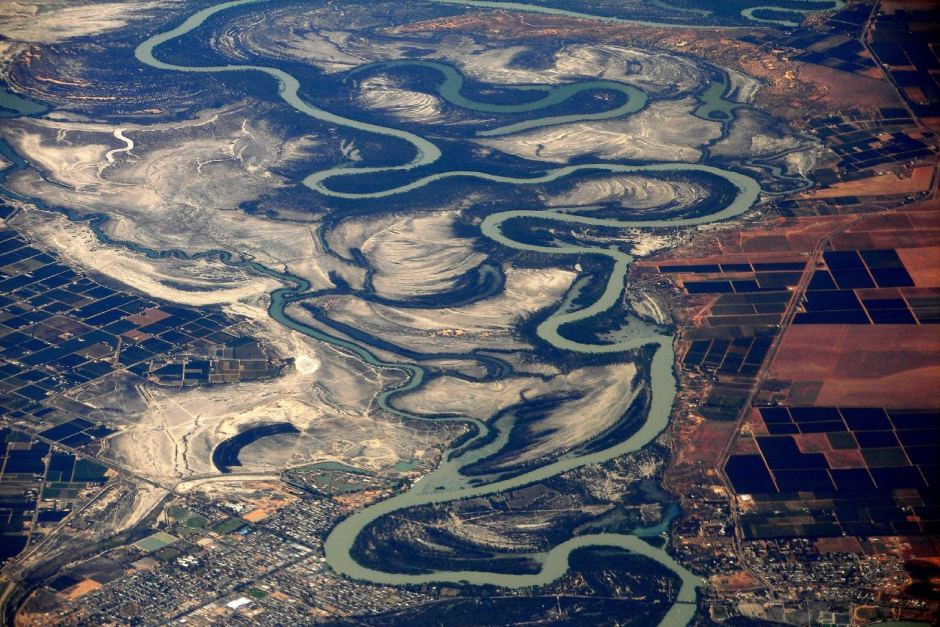
\includegraphics[width=1\textwidth]{01.9-water-murray-darling/figures/water_Murray-Darling-junction}
	\caption{Murray-Darling junction, Australia. Photo by: Michael Storer}
\end{figure}


The Murray-Darling Basin receives most of its rainfall from a very small percentage of the Basin; mainly along the southern and eastern parts. The rest of the basin is flat and low-lying, contributing very little or no run-off to the rivers. Relevant for this study, many tributaries within the basin are intermittent streams, with highly variable flows dependent on the wetness of the year.

\subsection{Study Site: Murray-Darling River Basin}
\begin{figure}[H]
	\centering
	\includegraphics[width=1\textwidth]{01.9-water-murray-darling/figures/Figure1}
	\caption{Overview of the study area, Murray-Darling River Basin, and vector water mask dataset extracted from OSM. The inset map is based on Natural Earth 1 raster dataset (\url{http://www.naturalearthdata.com/})}
	\label{fig:au-study-area}
\end{figure}

\subsection{Input datasets used to extract water mask}
Even though HydroSHEDS provides a much better coverage, its resolution is limited to 15 arc seconds (~450m), which is insufficient to resolve all small water features required for detailed water-related applications. Furthermore, it was based on older, 90m revision of \gls{SRTM}, which is less detailed compared to a recently released 30m version. Therefore, to develop a method to generate the water mask, we have used four input datasets (see Table \ref{table:au-datasets} and Figure \ref{fig:au-datasets}). The first dataset, Landsat 8, combines 2743 scenes of optical multi-spectral satellite imagery acquired during 2013-2015 over the study area. The Landsat 8 mission already operates for more than two years and, therefore, provides a reasonably long period of information to estimate water dynamics on a global scale. The second dataset is based on the new 30m revision of the \gls{SRTM} digital elevation model. The last data source consists of all water features, extracted from a recent version of OSM Planet File \citet{dataOSMPlanet}. Additionally, HydroBASINS \citet{Lehner2013} was used as a supplementary dataset to simplify extraction of a drainage network from \gls{SRTM}.

\begin{table}
	\centering
	\caption{Input datasets used for the analysis}
	\label{table:au-datasets}
	\small
	\begin{tabular}{| r | c | c | C{7cm} |}
		\hline
		\textbf{Dataset} & \textbf{Type} & \textbf{Resolution} & \textbf{Notes} \\ 
		\hline
		Landsat 8 TOA & Raster & 15m, 30m,60m & 2743 scenes were used acquired during 2013-2015, top of atmosphere (TOA) reflectance. \\
		\hline
		\gls{SRTM} & Raster & 30m & Effective resolution is lower due to the presenceof high-frequency noise \\ 
		\hline
		OpenStreetMap & Vector & 1m-100m & Planet file from August 2015, the following tagsquery was used to indicate water features:natural=water or natural=spring or waterway=or landuse=basin or landuse=reservoir orbarrier=ditch or landuse=saltpond \\
		\hline
		HydroBASINS & Vector & 450m & Level 8 basins were used to delineate \gls{HAND} using 30m version of \gls{SRTM} \\
		\hline
	\end{tabular}
\end{table}

Extraction of water features from OSM is a relatively trivial task, mainly consisting of a careful selection of proper filters and data conversion tools. We have used data conversion tools provided by OSM and a set of programs based on GDAL (\url{http://www.gdal.org/}) to select only relevant features representing surface water. 
To derive a high-resolution drainage network from \gls{SRTM}, we have used the D8 method \citet{OCallaghan1984}, implemented using PCRaster \citet{Karssenberg2010}. The stream delineation step was applied for every -catchment of the Murray-Darling basin. The HydroBASINS level 8 catchment geometries were used for this purpose. This step was required due to the large size of the catchment making it difficult to perform processing in a single step.

Extraction of the water mask using Landsat 8 imagery was the most challenging task and required the development of a new method to derive a water mask from multi-spectral imagery. The new method combines the use of the \gls{MNDWI} spectral index (\ref{eq:au_MNDWI}) extended with a non-parametric detection of a local threshold to improve the accuracy of water detection. The \gls{MNDWI} is very similar to the \gls{NDWI} spectral index (\ref{eq:au_NDWI}), but uses a short wave infrared band instead of near-infrared. Additional steps include the use of the \gls{NDVI} \citet{Tucker1979} (\ref{eq:au_NDVI}) with a high threshold value (0.3) to exclude false water detection in very dark vegetated areas. 

\begin{equation}
NDWI = \left(\rho_{green}-\rho_{nir} \right) / \left(\rho_{green} + \rho_{nir} \right)
\label{eq:au_NDWI}
\end{equation}

\begin{equation}
MNDWI = \left(\rho_{green}-\rho_{swir1} \right) / \left(\rho_{green} + \rho_{swir1} \label{eq:au_MNDWI}
\right)
\end{equation}

\begin{equation}
NDVI=\left(\rho_{nir} - \rho_{red}\right) / \left(\rho_{nir} + \rho_{red} \right)
\label{eq:au_NDVI}
\end{equation}

where $\rho_{green}$, $\rho_{swir1}$, $\rho_{nir}$, and $\rho_{red}$ represent TOA reflectance for corresponding Landsat 8 bands.

We have included an additional classification step to refine the water mask for hilly areas, where the results of automated classification led to high commission errors. We have used a supervised classification based on \gls{CART} \citet{Breiman1984}, which was trained using a manually digitized training set to distinguish between water and land pixels. 

\begin{figure}
	\centering
	\includegraphics[width=1\textwidth]{01.9-water-murray-darling/figures/Figure2}
	\caption{The datasets and their corresponding water masks: \gls{OSM} (A and D), Landsat 8 (B and E) and 30m \gls{SRTM} (C and F). Murrumbidgee River, north of Canberra.}
	\label{fig:au-datasets}
\end{figure}

Our selection of the input datasets was based on the assumption that the accuracy of all three datasets is similar. However, estimation of the actual errors of OSM would be difficult, mainly because OSM features are usually based on different measurement methods (GPS traces, manual digitizing using medium or high-resolution imagery of bulk import from other databases of varying nature). For Landsat 8 and \gls{SRTM} the main limitations are well known \citet{Roy2014}, \citet{Rodriguez2006}. Horizontal accuracy of Landsat 8 is known to be better than 12m in 90\% of the 30m resolution images of the Operational Land Imager (OLI). For \gls{SRTM}, vertical relative and absolute errors can be explained by its radar nature and are in the order of 10 and 16 meters for 90\% of the data, with an absolute geolocation error below 13m. 

\subsection{Derivation of hydrological variables: drainage network and HAND}
In addition to the drainage network, a number of other hydrological parameters were derived during \gls{SRTM} analysis, such as local drainage direction, flow accumulation, and \gls{HAND} (see Figure \ref{fig:au-dem-hand}). 

A (potential) water mask was generated by thresholding \gls{HAND} values using 1m elevation above the nearest drain. We found this approach to work better in estimating water masks in flat areas compared to the methods based on flow accumulation.

All hydrological variables were derived using the following steps: 1) clip DEM using a Google Earth Engine script and one of 1494 HydroBASIN polygons and download it to Google Compute Engine (GCE); 2) Compute slopes, local drainage directions (LDD, includes pit-removal step), flow accumulations, and \gls{HAND}. 3) Upload results to Google Earth Engine (\url{http://earthengine.google.com}) and Google Fusion Table (\url{http://tables.googlelabs.com/}) so they can be used in parallel processing scripts for further analysis. To compute \gls{HAND}, a drainage network had to be estimated by thresholding the flow accumulation. We have used a threshold equal to 100 upstream cells, which was sufficient to detect most of the potential rivers. 

\begin{figure}
	\centering
	\includegraphics[width=1\textwidth]{01.9-water-murray-darling/figures/Figure3}
	\caption{Digital elevation model, \gls{SRTM} 30m (left) and \gls{HAND} (right).}
	\label{fig:au-dem-hand}
\end{figure}

The resulting \gls{HAND} can be used for the estimation of potential flood areas, but also to detect pixels where potential errors occur due to hill shadows. These areas were estimated by generating a binary mask based on a variation of \gls{HAND} values. The mask showing potential hilly areas was computed by marking pixels as hilly in a case where \gls{HAND} values larger or equal to 30m were found in the 300m radius neighborhood.

\subsection{Method of water detection using Landsat 8}

Our method of water detection from multi-spectral multi-temporal imagery is based on a step-wise approach combining unsupervised and supervised classification steps (Figure \ref{fig:au-pipeline}). The unsupervised step was applied first to detect the initial water mask using percentile images of reflectance, resulting in minor omission errors in flat areas. However, we obtain very high commission errors in hilly areas due to terrain shadow. Therefore, an additional step was required to refine the water mask using supervised classification. The unsupervised classification step is based on the local adaptive threshold detection method presented in Chapter \ref{ch3}. 

\begin{figure}[H]
	\centering
	\includegraphics[width=1\textwidth]{01.9-water-murray-darling/figures/Figure9_1}
	\caption{Optimal threshold computed around potential surface water edges}
\end{figure}

\begin{figure}[H]
	\centering
	\includegraphics[width=1\textwidth]{01.9-water-murray-darling/figures/Figure7}
	\caption{False-color intensity percentile composite image (swir1, nir and green) (left), \gls{MNDWI} index values (middle) and its histogram (right)}
\end{figure}

\begin{figure}[H]
	\centering
	\includegraphics[width=0.8\textwidth]{01.9-water-murray-darling/figures/Figure8}
	\caption{Water boundary classified using threshold = 0.0 (left) and threshold = 0.32 automatically detected for this location using new method (right).}
	\label{fig:au_river_water_hist}
\end{figure}

The proposed method was applied to the cloud-free percentile images. In a case of two classes in the grid tile, we were able to get an almost perfect detection of water pixels using the following parameters: s=0.7,th=0.99 for the Canny edge filter, and a structuring element with the size 15m x 15m to dilate the edges in step 3 and create a surrounding buffer region. The \textit{s} and \textit{th} parameters are used to define the standard deviation of the Gaussian smoothing kernel and the threshold used to define sensitivity of the filter, respectively.

\begin{figure}
	\centering
	\includegraphics[width=1\textwidth]{01.9-water-murray-darling/figures/Figure10}
	\caption{Histograms of \gls{MNDWI} values within 15m of detected edges (A) and a histogram of detected threshold values (B)}
	\label{fig:au-ndwi-values}
\end{figure}

\subsection{Refining water detection using supervised classification based on CART and HAND}
The method was applied over 1725 spatial boxes of 20km x 20km covering the Murray-Darling basin. The 20x20 km area was chosen arbitrarily, and it is assumed that the threshold values are the same within each spatial box area. The resulting \gls{MNDWI} threshold values have a range of -0.25 to 0.4 (Figure \ref{fig:au-ndwi-values}), which clearly highlights the need for varying the \gls{MNDWI} threshold spatially. 

The supervised classification step, based on \gls{CART}, was introduced to reduce commission errors found in the case of shadows and snow/ice pixels. It was performed only for hilly areas where misclassified pixels were observed. Hilly areas were detected using a threshold of Hmax, representing the minimum \gls{HAND} value (30m in our case). In this way, we could keep omission errors low for flat areas and ensure low commission errors for hilly areas. The final error of water detection was very low (less than 1\%), mainly due to a presence of mixed pixels or incomplete training data for hilly areas. An additional step was required to exclude very dark vegetated areas, resulting in high \gls{MNDWI} values and, therefore, misclassified as water. These errors were removed by eliminating pixels with \gls{NDVI} values greater than 0.3.

\begin{figure}
	\centering
	\includegraphics[width=1\textwidth]{01.9-water-murray-darling/figures/Figure4}
	\caption{Water detection processing pipeline}
	\label{fig:au-pipeline}
\end{figure}

In order to compute the final water mask, the study area was divided into regular grid tiles of 0.2 x 0.2 degrees in size. This step was needed to make sure that the dynamic \gls{MNDWI} threshold is estimated for every tile, but also to parallelize the processing. Finally, the above workflow was applied for every tile.

\subsection{Cloud-free Landsat 8 percentile images}
Our method to exclude clouds and shadows in the satellite imagery is based on the use of percentile images extracted from an image collection, spanning a two year period (2013-2015), instead of the original images. The percentile images were computed on a per-pixel and per-band basis using 50-130 top of atmosphere (TOA) intensity values. The larger number of images comes from a higher revisit frequency due to an overlap in the satellite swath. 

\begin{figure}
	\centering
	\includegraphics[width=1\textwidth]{01.9-water-murray-darling/figures/Figure5}
	\caption{Intensity percentile false-color image (swir1, nir, green) based on 2743 Landsat 8 images for 2013-2015, 20\% (left), 50\% (middle), 80\% (right)}
	\label{fig:au-percentiles}
\end{figure}

The percentile images (Figure \ref{fig:au-percentiles}) appeared to describe the water dynamics in a better way than the interval mean images used in other studies \citet{Potapov2012}, \citet{Hansen2013}. Evensthough we have confirmed this result only by visual inspection, the reasoning comes from the fact that the water surface area may change sharply depending on local topographic conditions. This water area change results in sharp changes between water masks present in different percentiles (see Figure \ref{fig:au-percentiles-clouds}). 

\begin{figure}
	\centering
	\includegraphics[width=1\textwidth]{01.9-water-murray-darling/figures/Figure6}
	\caption{Intensity percentile false-color (swir1, nir, green) images. Left to right: 5\%, 10\%, 20\% for areas with average cloud cover 32\% (top) and 4\% (bottom). }
	\label{fig:au-percentiles-clouds}
\end{figure}

Over the Murray-Darling basin, the percentile range of 15\%-55\% of all TOA intensities was empirically found to be suitable for permanent water detection. However, for semi-arid and flat areas, where cloud frequency is very low, a larger range of percentiles (up to 90\%) could be used as well. Average images generated for very low percentiles usually result in too many artifacts present in the images due to cloud and hill shadows, making them difficult to interpret automatically (Figure \ref{fig:au-percentiles-clouds}) top/left. At the same time, the use of lower percentiles has a higher chance to represent a larger amount of surface water, present during floods and wet seasons and a smaller amount of surface water observed during dry seasons (bottom row with cloud frequency = 4\%). For a more detailed analysis the choice of the upper and lower percentiles can be estimated by taking cloud frequency and topographic conditions into account.

The use of simple water spectral indices in hilly areas is usually not sufficient, as they frequently result in very high commission errors due to false detection of water pixels. This misclassification is especially true for \gls{MNDWI}, which is more sensitive to hill shadows than \gls{NDWI}. The reason is the spectral signature of hill shadows, which looks similar to the one corresponding to water, resulting in large \gls{MNDWI} values. To remove these errors, we have trained a \gls{CART} classifier using a manually created training set, all Landsat 8 bands, and \gls{HAND}. The training set was created only to include those pixels that were misclassified during the unsupervised step, which appeared to be true only in hilly areas. The \gls{HAND} values used to train the classifier were included only when they were greater than 10m. This constraint was introduced to reduce the influence of \gls{SRTM} errors that get higher near water bodies.

The classification was performed using a Google Earth Engine implementation of \gls{CART} with a tree depth increased from 10 (default value) to 20. The larger tree depth was required to avoid overfitting and because our study basin covers a relatively large area, resulting in a large variation of water and land use types. Overfitting was detected by observing the confusion matrix generated after training the classifier. In the final training set, the confusion error was very close to zero. 

\begin{figure}[H]
	\centering
	\includegraphics[width=1\textwidth]{01.9-water-murray-darling/figures/Figure11}
	\caption{Steps performed during supervised classification post-processing step for hillslope areas. (tile 2847). False color 15\% percentile composite image (A), \gls{MNDWI} scaled from (B), water detected using adaptive threshold method (C), results of application of \gls{CART} classifier (D), 300m buffer areas around HAND > 30m used to select final water mask (E) and the final water mask (F).}
\end{figure}

The final training set contains about 500 polygons created manually and iteratively by training the classifier for one set of tiles and then validating it for all other tiles where supervised classification was required. This step was required mainly for the grid tiles located in the southern part of the catchment (hilly landscapes).

Since Landsat can reveal water features better than \gls{SRTM}, we have also decided to analyze the \gls{HAND} values of all pixels used during the training stage (Figure \ref{fig:au-hand-vs-mndwi}). The results reveal that \gls{HAND} values can take values up to 40m even though visual inspection shows that these pixels belong to water. A low \gls{SRTM} accuracy can explain this mismatch near water. Another confusing result comes from a comparison of \gls{NDWI} and \gls{MNDWI}. Theoretically, they should be strongly correlated. However, substantial differences were observed in multiple locations. These differences occur because many pixels requiring manual classification are mixed pixels, partially covered by land. Further research would be necessary to explain these results.

\begin{figure}[H]
	\centering
	\includegraphics[width=1\textwidth]{01.9-water-murray-darling/figures/Figure12}
	\caption{Values of \gls{HAND} vs. \gls{MNDWI} (A) and \gls{MNDWI} vs. \gls{NDWI} (B) used during training of CART classifier. Orange and blue dots represent land and water correspondingly}
	\label{fig:au-hand-vs-mndwi}
\end{figure}

\subsection{River centerline estimation from Landsat 8 water mask}
An additional skeletonization step was required before computing positional differences between OSM linear water features and water masks detected from Landsat imagery (or \gls{HAND}). We have used the method of mathematical morphology \citet{Serra1982} by applying an iterative thinning operator applying a hit-or-miss transform to a binary water mask image. The actual steps include:

\begin{equation}
S(W)=\bigcap_{k=0}^K \left(W \otimes kB \right)
\end{equation}

where $\otimes$ is a binary thinning operator defined as:

\begin{equation}
W \otimes B = W - \left( W \odot B \right)
\end{equation}

where $\otimes$ is a hit-or-miss transform operator defined as:

\begin{equation}
W \odot B = \left( W \ominus B_1 \right) \bigcap \left( W_c \ominus B_2 \right)
\end{equation}

The structuring elements $B_1$ and $B_2$ used for skeletonization (Figure \ref{fig:au-skeleton}) allow reconstruction of river skeletons even without the need to introduce pruning (the removal of small branches), which is usually required during such processing. The actual implementation performs a hit-or-miss transform using four rotated versions of the structuring elements applied sequentially during every thinning operation.

$W_c$ denotes a set complement of $W$, referring to elements not in $W$. 

Additionally, morphological smoothing was performed before the skeletonization step, to make sure fewer branches were present in the final centerline.

\begin{figure}
	\centering
	\includegraphics[width=1\textwidth]{01.9-water-murray-darling/figures/Figure13}
	\caption{Input water mask (left) and results (right) of medial axis detection algorithm using mathematical morphology. Structuring elements (kernels) shown in the middle}
	\label{fig:au-skeleton}
\end{figure}

To implement most algorithms, we have used the Google Earth Engine (GEE) parallel computing platform \citet{Gorelick2012}. Some of the computations, where GEE was less suitable, were performed using Google Compute Engine (GCE) running Ubuntu 15.04 (Vivid Vervet). The use of a dedicated machine was more suitable for the computation of hydrological parameters from the DEM, for which no algorithms are available yet in the GEE environment. JavaScript and Python were used as programming languages, as well as some open-source tools and libraries (GDAL \citet{GDAL}, Fiona \citet{webFiona}, Shapely \citet{webShapely}, ee-runner \citet{webEErunner} and PCRaster \citet{Karssenberg2010}). We aimed at automating most of the steps to make sure that they would easily scale to a planetary scale, and that the results of the research can be reproduced when updated versions of the underlying datasets will be released.

\section{Results}
\subsection{Estimation of positional differences between rivers}
After the centerline is computed, positional differences can be easily computed using the Goodchild’s method of increasing overlay polygons.

\begin{figure}
	\centering
	\includegraphics[width=1\textwidth]{01.9-water-murray-darling/figures/Figure14}
	\caption{Method used to estimate positional differences between vector and raster datasets. Increasing overlay buffer method (A), example of OSM water polyline and Landsat mask (B), results for two different buffer sizes (C, D)}
	\label{fig:au-positional-accurracy-method}
\end{figure}

The above method works best when the lengths of the segments and the distance between segments are significantly larger than the maximum buffer size $D_{bmax}$ used during dilation. 

\section {Positional differences between OpenStreetMap, Landsat, and SRTM}
The Goodchild’s method to estimate positional differences was applied for every line segment of the OSM dataset and two water mask raster datasets: 1) drainage network estimated using \gls{HAND} and 2) water centerline estimated using Landsat 8 water mask. The final differences were estimated using Score = 0.85 as a threshold, which corresponds to a distance where 85\% of the pixels from the second dataset (black line in Figure \ref{fig:au-positional-accurracy-method}) are covered by a dilation via this distance. The frequency and cumulative histograms of the resulting differences are presented in Figure \ref{fig:au-positional-differences}. 

\begin{figure}
	\centering
	\includegraphics[width=1\textwidth]{01.9-water-murray-darling/figures/Figure15}
	\caption{Frequency histogram of distances between OSM river segments, Landsat 8 centerline, and \gls{SRTM} (30m) drainage network.}
	\label{fig:au-positional-differences}
\end{figure}
 
The second peak of the left histogram (distance > 100 m) occurs mainly due to wider water bodies, where the centerline cannot be reached within 20 thinning steps, but also for water bodies that start to overlap within the maximum size dilation, such as oxbows or meandering rivers located close to each other.  Positional differences between Landsat centerlines and OSM become larger when a river width becomes larger. These large differences are observed because OSM polylines frequently represent the thalweg (the line of lowest elevation within a river) instead of a medial axis.

It can be seen that the distance between OSM water polylines and the centerlines computed using the Landsat 8 water mask falls in the range of 30-60 meters for 60\% of the water features. We were able to confirm this for about 17\% (N=5687) of the linear OSM water features. The length of the river segments was selected to be about 0.02 degree (~2.2 km). 

In the case of \gls{SRTM}, about 30\% (N=9887) of the OSM segments could be compared, mainly located in the southern, hilly part of the catchment (see Figure \ref{fig:au-positional-differences-map}). The distances are slightly larger than those for LANDSAT, and also appear normally distributed with a mean value of 110 meters. This may be explained by a systematic shift between the OSM and \gls{SRTM} datasets, combined with other factors, like the fact that smaller river meanders were not resolved well by \gls{SRTM} dataset.

\begin{figure}
	\centering
	\includegraphics[width=1\textwidth]{01.9-water-murray-darling/figures/Figure16}
	\caption{Positional differences between linear water features extracted from OSM, water mask centerline extracted from Landsat (left) and drainage network extracted from \gls{SRTM} (right)}
	\label{fig:au-positional-differences-map}
\end{figure}

Spatial representation of the distances between OSM river segments and centerlines of the LANDSAT water mask, as well as the distances between OSM river segments and drainage network cells, are shown in Figure \ref{fig:au-positional-differences-map}. It can be clearly seen that, in the case of Landsat, mainly large rivers could be compared due to the 30m resolution limitation of the OLI sensor. At the same time, a much larger number of the OSM segments could be confirmed using the drainage network derived from 30m \gls{SRTM}, even though positional differences are not as good as in the case of LANDSAT. On the other hand, the drainage network derived from \gls{SRTM} seems to be very inaccurate for flatter landscapes. Therefore, we have excluded drainage network pixels for the cases where \gls{HAND} values are smaller than 30m in the 300m radius neighborhood. These parameters were identified empirically after careful visual inspection.

\subsection{Goodness of fit between OpenStreetMap and Landsat water masks}
To estimate the overall overlap between water masks extracted from both OSM and Landsat, we have aggregated the overlap using a regular grid for a better understanding of the results. The analysis was performed using the actual water mask (polygonal and linear features of the OSM). For every grid cell, a total surface area of water mask was computed. For linear features, a dilation buffer of 15m was applied using a square kernel to make sure it matches, at least, one Landsat grid cell. Then, the resulting thematic differences were computed (Figure \ref{fig:au-positional-differences-thematic}).

\begin{figure}
	\centering
	\includegraphics[width=1\textwidth]{01.9-water-murray-darling/figures/Figure17}
	\caption{Thematic differences between water surface area provided by OSM and detected using Landsat 8}
	\label{fig:au-positional-differences-thematic}
\end{figure}

While the centerline analysis reveals a good fit between Landsat and OSM, the surface area analysis demonstrates quite a large mismatch. There can be several explanations for this mismatch. Firstly, OSM (as well as Google Maps) misses a large number of small agricultural reservoirs in this area. Secondly, many of the large reservoirs are intermittent and were mostly dry during 2013-2015. Thirdly, river bank information frequently does not match between two datasets; in some cases it is missing in OSM, in other instances, Landsat misses small rivers (W < 30m) or the water bodies are partially covered by vegetation.

\begin{figure}
	\centering
	\includegraphics[width=0.75\textwidth]{01.9-water-murray-darling/figures/Table3}
	\caption{Overlap between surface water detected using OSM and Landsat}
	\label{fig:final-overlap}
\end{figure}

The surface water area of both OSM and Landsat constitutes about 0.85\% of the total catchment area. Only about one-third (32\%) of the total surface water area can be observed using both datasets. The rest of the surface water can be seen using only Landsat or only OSM (Figure \ref{fig:final-overlap}).

\section{Supplementary Materials}
All scripts used in this chapter, including training set used for water mask refinement in hilly areas, can be found on the following GitHub repository: \url{http://github.com/gena/paper-osm-2015}. The repository contains all scripts which allow to: 1) extract water features from \gls{OSM} planet file; 2) download \gls{SRTM} files clipped by HydroBASIN catchments and perform calculation of \gls{HAND} using Python version of PCRaster tools; 3) Google Earth Engine JavaScript scripts used to generate regular grid for processing, detect water mask for a given grid tile as well as scripts required to skeletonize that water mask and compute distance between OSM segments and another river raster dataset (drainage network derived from \gls{HAND} or Landsat water mask centerline). Additional supplementary scripts are available in Jupyter Notebooks. These scripts were used to clean-up HydroBASINS catchments, generate tiled version of \gls{HAND} from basin-based images, split \gls{OSM} water geometries into smaller segments to perform local spatial analysis as well as scripts used to generate histograms from GeoJSON files produced by water detection scripts.

\subsection{Grids used during analysis}

The following two grids were used during analysis: 1) HydroBASINS level 8 catchment polygons 2) regular ~20x20km grid. The first one was used to parallelize generation of hydrological parameters. The latter one was used to perform water detection and to visualize the results in an aggregated form, and to parallelize the water detection analysis using Landsat imagery.

\begin{figure}
	\centering
	\includegraphics[width=1\textwidth]{01.9-water-murray-darling/figures/Figure18}
	\caption{HydroBASINS Pfafstetter level 8 catchments (left) and regular ~20x20km grid}
\end{figure}

\subsection{Results as raster and vector datasets}

Some of the datasets used during processing were uploaded and shared as Google Fusion Tables and Google Earth Engine Raster Assets, including:


\begin{table}
	\centering
	\caption{List of vector and raster datasets available online}
	\label{table:au-datasets-output}
	\small
\scalebox{0.7}{
	\begin{tabular}{| c | c | C{9cm} |}
		\hline
		\textbf{Name} & \textbf{Type} & \textbf{Link} \\ 
		\hline
		OpenStreetMap water features & Fusion Table & \url{http://bit.ly/paper-osm-2016-fusion-tables} \\
		\hline
		HydroBASIN catchments	& Fusion Table & \url{http://bit.ly/paper-osm-2016-fusion-tables} \\
		\hline
		Landsat water mask	& EE Asset 	& users/gena/AU\_Murray\_Darling/MNDWI\_15\_water\_WGS \\
		\hline
		HAND & EE Asset 	& users/gena/AU\_Murray\_Darling/SRTM\_30\_Murray\_Darling\_hand \\
		\hline
		Local flow accumulation & EE Asset & users/gena/AU\_Murray\_Darling/SRTM\_30\_Murray\_Darling\_flow\_accumulation \\
		\hline
		Distance to the nearest drainage & EE Assets & users/gena/AU\_Murray\_Darling/SRTM\_30\_Murray\_Darling\_dist \\
		\hline
		Google Earth Engine script & JavaScript & \url{http://bit.ly/paper-osm-2016-gee-assets} \\
		\hline
	\end{tabular}
}
\end{table}

\section{Website}

\begin{comment}
\begin{figure}
	\centering
	\includegraphics[width=1\textwidth]{01.9-water-murray-darling/figures/Figure19}
	\caption{A screenshot of the website demonstrating water mask derived from Landsat 8, \gls{OSM} and 30m \gls{SRTM}}
\end{figure}
\end{comment}

Most of the datasets produced by this research can be accessed using a website (\url{http://osm water.appspot.com}) dedicated to this study. The website is hosted in a Google Cloud and uses Google App Engine infrastructure, providing integration with Google Earth Engine where most of the datasets produced in this study can be found.

\section{Conclusions and Discussion}
The research demonstrates clear benefits of the use of the new imagery acquired by Landsat 8 to detect water bodies when combined with water masks derived from other sources. We have also found the \gls{SRTM} to be an excellent complimentary dataset enabling improvement of the water mask detection method for hilly areas, after its transformation into \gls{HAND}.

However, none of the three water masks was found to be perfect regarding positional differences and completeness. The main issue of the water masks derived from Landsat 8 is its shortcomings in detecting small water features such as small rivers or man-made canals and detecting water bodies (partially) covered by riparian or surface water vegetation. The main limitation with the drainage network derived from \gls{SRTM} is its inability to detect river features for flat terrain conditions. The latter constituted a major part of our study area. An additional challenge is related to the presence of high-frequency noise and a relatively poor quality of \gls{SRTM} near water bodies. The noise can be explained by the radar origin of the dataset. 

One of the next logical steps of the present research could be the development of a data fusion algorithm using the strengths of all three datasets. Such development would require the introduction of objective criteria regarding confidence of every water mask depending on topographic and other conditions. Another step might be to perform the same analysis globally. However, performing global analysis would require significantly larger computational efforts and includes both detection of the water mask and estimation of \gls{HAND} at 30m resolution. Additional validation of the OSM and its fusion with the datasets produced by the local governmental agencies (Surface Hydrology, Water Observations from Space, local high-resolution elevation models) will help harmonizing existing vector and raster water mask datasets.

Possible improvements to the method of water detection might include utilization of the panchromatic band and entropy-based methods in addition to the spectral methods. Additional significant improvements can be achieved through the use of the other medium or high-resolution satellite missions such as Sentinel 2, PlanetLabs and SkyBox. The use of higher resolution imagery would allow detection of much smaller (width < 30m) river features, resulting in improved coverage.
The method of water detection can be easily extended to use Landsat 7 or any other multi-spectral imagery, for example, to generate an inter-annual water mask or to study water dynamics. 

The proposed method of water detection might face difficulties in the areas where an insufficient number of cloud-free observations is available, for example, in very wet or cold climates. In this case, it might be difficult to determine a correct range of the cloud-free percentiles to be used for water detection. 
